\chapter{Introduction}
\label{Ch:Introduction}

%\chapter{Introduction}
%\subchapter{Unmanned Aerial Vehicles and Their Integration into the Civil Airspace System}
\section{Unmanned Aerial Vehicle and the Civil Airspace System}
\label{S:UAVandCivilAirspace}

\lettrine[lines=3, nindent=0pt]{U}{nmanned} Aerial Vehicle (UAV), or Uninhabited Aerial Vehicle, or Unpiloted Aerial Vehicle, or Unmanned Aircraft, or drone, is defined as a device that is used for flight in the air that has no human on-board and is controllable in its three axes. Therefore, all classes of airplanes, helicopters, airships, and translational lift aircraft are included in this definition, while kites and traditional balloons [REF] are excluded. The history of UAVs hence can be stretches back as far as in March 1917, when Archibald’s Ruston Proctor AT (Aerial Target) was launched using compressed air from a back of a lorry at Upavon Central Flying School near Salisbury Plain, shown in Figure~\ref{f:UAVHistory}-a [REF]. Separately in March 1918, the first Curtis-Sperry remote controlled ‘Flying Bomb’ was also launched (see Figure~\ref{f:UAVHistory}-b) from the top of a Marmon automobile driving along the Long Island Motor Parkway, New York. Afterwards, the UAV technology grew throughout the period of First World War, particularly for those two purposes, as an Aerial Target (later known as target drones) and a Flying Bomb (later known as guided missiles). Around 20 years later, the first UAV usage outside the military ground was demonstrated, when Ross Hull and Clinton B DeSoto built and flew their remote controlled model planes in 1937, as shown in Figure~\ref{f:UAVHistory}-c. The military, however, continues to be the center of UAVs advancement, expanding their usability for intelligence, surveillance, target-acquisition, and reconnaissance.
%It was also in the 1990s that a more peaceful role for UAV systems was conceived. Scientific endeavors, such as persistent environmental monitoring, were seen as ideal function for UAVs. The solar-powered Pathfinder and Helios aircraft, both developed by NASA and the Aerovironment Corporation in the late 1990’s, exemplified the development of innovative research UAVs. Other countries also began to develop UAVs for non-military applications. For example, in 1998 an Australian firm produced a 30 pound UAV, called the Aerosonde Laima, which crossed the Atlantic Ocean autonomously on only 1.5 gallons of automotive gasoline.

\begin{figure}
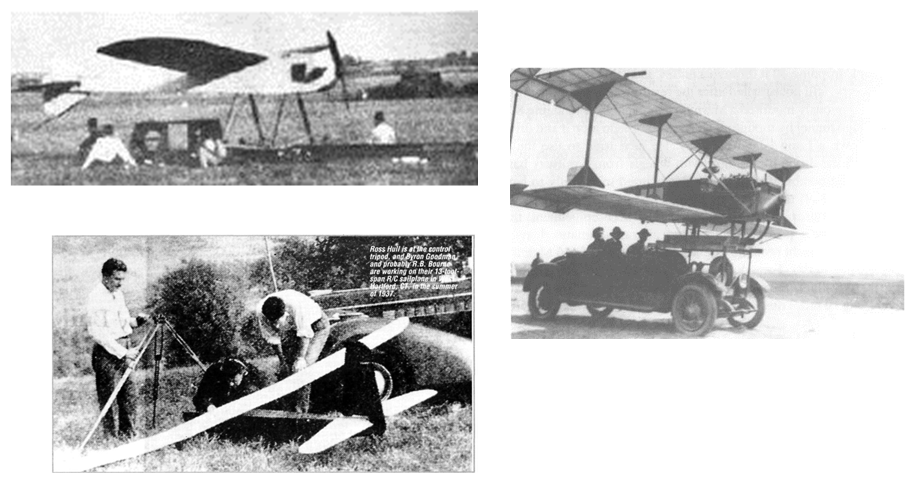
\includegraphics[width=1\textwidth]{\TheDir Figures/UAVHistory}
 \caption{The pioneers of Unmanned Aerial Vehicle Technology (a) Archibald's Ruston Proctor AT, (b) Curtis-Sperry 'Flying Bomb', and (c) Ross Hull and Clinton B DeSoto remote controlled model plane.} 
\label{f:UAVHistory}
\end{figure}

Not until recently the commercial values of UAVs for civil purposes are widely recognized, thanks to advancement of technology in materials, sensors, computation, and telemetry. As UAVs become much cheaper and more controllable, many are motivated to incorporate them in their everyday business. DeGarmo [REF] introduced seven examples of UAVs prospective for civil applications, as illustrated in Figure~\ref{f:ProspectiveUAV}. Retail companies, for example, could offer a drone delivery service to their customers [REF], media could obtain aerial footage of an incident immediately using a UAV [REF], and hospitals could send by drone a heart defibrillator to a rural location[REF]. Similarly, Information Technology companies might want to launch a high-altitude imagery drone to update their online map services [REF], theme parks could incorporate a drone as a flying dancer UAVs to join its performance shows[REF], and countless other possibilities. 

\begin{figure}
\begin{center}
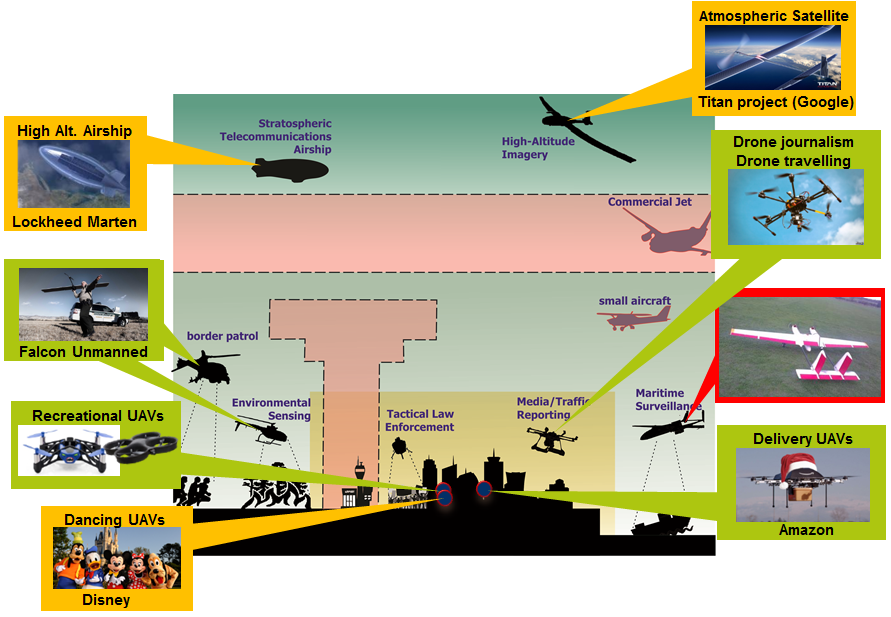
\includegraphics[width=0.8\textwidth]{\TheDir Figures/ProspectiveUAV}
\end{center}
\caption{Prospective commercial applications of UAVs integrated in the airspace system, adapted from the work of \cite{degarmo:04} with addition.} %Ref.\cite{barfield:00} and \cite{Jenie:13a}.}
\label{f:ProspectiveUAV}
\end{figure}

All of those prospective applications can be achieved once UAVs are fully integrated into the civil airspace system, which, however, is not yet the case. UAV flights are currently considered unsafe and only allowed in a pre-permitted segregated area from the airspace system. UAV operations can create a whole new traffic in the airspace system that, if it is not managed, could be hazardous for the current manned air traffic, the people on the ground, and the general environment. This view contributes to the reluctance of most airspace authorities to provide adequate regulations for civil UAV operation beyond the line-of-sight\cite{CAP722}. In the United States, it is generally forbidden to fly drones commercially [REF], while recreational drones have several limitations. The United Kingdom allows the operation of UAV that weigh less than 20 kg without any airworthiness approval, but requires pilot certification[REF]. In the Netherlands, a UAV that is flown commercially or professionally need to have its airworthiness and its pilot approved and registered, while amateurs (hobbyist) can fly anywhere below 1000 feet and more than 150 meters from any public buildings [REF]. Most parts of Asia, such as Singapore or Indonesia, currently have no specific restriction on any UAV activities, except if it violated the general public policies [REF].

Therefore, the problem of safe integration into the Airspace System has been a major topic in UAV research for at least the last decade [REF]. The problem differs from manned flight domain: instead of protecting the vehicle itself, safety in UAV is more about protecting the environment from the UAV. N.A. Sabatini[REF], the associate administrator for aviation safety, uses the “First, do no harm” principle, taken from the Hippocratic Oath of the medicine practices. Similarly, Barfield\cite{barfield:00} analogously describes the rule for UAV integration using the three laws of robotic featured in Robert Asimov famous science-fiction novel, “I, Robot”, which put the man (or manned) counterpart as the top priority in any safety procedures. The existing manned-flight and the people on the ground are the main concern when discussing the safety of UAV integration into the airspace system. Safety among UAVs, on the other hand, should be resolved with respect to those main subjects. 


\section{Problem Definition}
Any integration problem can be traced back to the level of readiness of the involved parties: the current airspace system and the new (future) UAV operations. Safe integration, therefore, can be achieved if the safety system in both domain is ready and compatible. This, however, is not yet the case since the two domains have been advancing separately in both research and practice. It is a chicken and egg situation - authorities and the public are reluctant to allow UAV flight in the airspace since they consider their CD\&R system is not ready, while UAV, as well as manned-flight, cannot focus more on maturing an integrated system since UAVs are not allowed to fly in a real airspace operation to gain experiences.

In manned-flight domain, the term 'Conflict Detection and Resolution' (CD\&R) is used to describe all systems and subsystems that mitigate conflict and collision, which includes hardware and software, off or on-board. This term, however, is uncommon in UAV domain. Most UAV research uses the term Collision Avoidance System (CAS) to represent such system. Many other terminologies that are commonly used in manned-flight are not used, or used differently, in the UAV domain. For instance, the acronym ACAS, which stands for Airborne Collision Avoidance System in manned-flight domain[REF], is used as an acronym for Autonomous Collision Avoidance System in many UAV studies[REF]. The terminology confusion perhaps reflects the gap between unmanned and manned flight researcher. This is elaborated more in the following sections.
%The different of term might be the underlying reason. Put it here!! below, juist descirbe the system, no term. Below, problem of architecturem risk, and UAV algorithm.

\subsection{Manned Flight's Conflict Detection and Resolution System}
Manned-flight CD\&R systems are managed in a fail-safe architecture, commonly known as the Layers of Safety, as it can be observed in Figure~\ref{f:MannedLayer}\cite{Dalamagkidis:09}. This architecture was not formed instantly; rather, it was built and iterated throughout history, where most of its components exist as the result of evaluations on accidents\cite{Kochenderfer:12}. Each of the layer of safety is regulated and therefore mandatory for every commercial flight, with only few exceptions. This architecture also serve as a guideline for further development of the CD\&R system in manned-flight.

\begin{figure}[h!]
	\begin{center}
		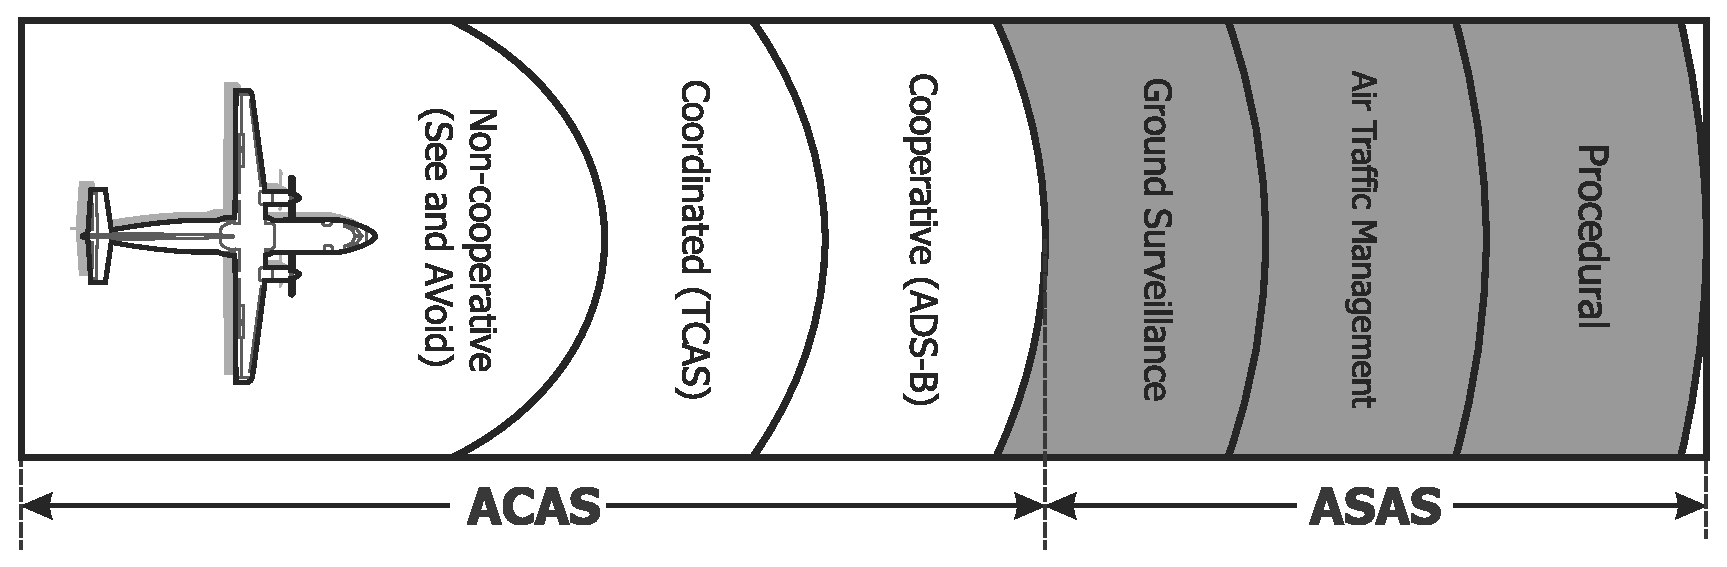
\includegraphics[width=0.8\textwidth]{\TheDir Figures/MannedLayer}
	\end{center}
	\caption{Manned flight Conflict Detection and Resolution Architecture (Layers of Safety)} %Ref.\cite{barfield:00} and \cite{Jenie:13a}.}
	\label{f:MannedLayer}
\end{figure}

The architecture is divided into two groups, i.e., the Airborne Separation Assurance System (ASAS) and the Airborne Collision Avoidance System (ACAS), shown in Figure~\ref{f:MannedLayer}. ASAS is long-range systems that maintain standard en-route separation between aircraft (typically 5 nautical-miles horizontal and 1000 feet vertical). Manned-flight achieves this separation by following the flight procedures, the Air Traffic Management directives, and by constant surveillance from the ground. ACAS, on the other hand, describes short range systems intended to prevent actual metal-on-metal collisions\cite{Hoekstra:01}. Here, the Traffic Warning and Collision Avoidance System (TCAS) have been used since 19--\cite{Kochenderfer:12}, while a more flexible system, the Automatic Dependent Surveillance Broadcast (ADS-B) is introduced recently[REF]. The last layer, the ‘see and avoid’, is essentially the pilot capability of avoiding any remaining obstacles that penetrate previous layers.

%readiness, compatibility
Since the current airspace system is dominated by the manned-flight, it is logical for UAVs to adapt directly this architecture in order to speed up their integration process. However, this architecture neglects several key characteristics of a UAV flights. For example, the first three layers implied that the aircraft should fly within the surveillance range of a ground station, while UAVs commonly designed to exploit rural area away from such station. The nature of materials used for UAV airframes is also a problem for ground surveillance, since mostly they are not traceable with RADAR. The architecture also only represent the variation of sensor use extensively in UAVs, in just one 'See and Avoid' layer. These problems leads to a need for a new CD\&R architecture that should be compatible and without changing the current manned-flight architecture.
%Problem 1: new architecture
\begin{tcolorbox}[colback=blue!5,colframe=blue!70!black,sharp corners=all,enlarge left by=5mm,width=120mm,title=\textbf{Problem 1}]
What kind of architecture can be defined to manage the Conflict Detection and Resolution system for UAV operation in an integrated airspace system? %How can the risk of the integration be defined, especially on interaction with manned-flight?
\end{tcolorbox}

%RISK -Problem 2


\subsection{UAV's Autonomous Collision Avoidance System}
Different than the manned-flight CD\&R system, UAV collision avoidance systems (CAS) are not regulated that every type of UAV might have its own method for avoidance. The situation actually results in rapid development of various avoidance approaches in both hardware and software. The research in this domain mostly focuses more on autonomous avoidance in as preparation for UAV operation beyond the line of sight of the operator.

Autonomous CAS for UAV can be elaborated in two branches of research, i.e., detection and resolution. UAV research in conflict detection mainly focuses on on-board sensors, either passive sensors such as cameras\cite{Fasano:08}, microphones [REF], or active such as a ultrasonic sensor[REF], laser range finder\cite{Hrabar:11} and RADAR\cite{Moses:14}. Filtering algorithms, such as the Kalman Filter[REF], have also been developed to compensate any inherited errors a that sensor always has. Collision resolution research, on the other hand, commonly focuses on the algorithms that are adapted from the general robotic domain, including the global and local path planning [REF], Voronoi diagrams [REF], potential field [REF], Optical flow [REF], Behavior [REF], Evolutionary [REF], and velocity obstacle [REF]. Only a few studies in UAV domain focuses on the development of the computational system on-board [REF].

While many collision avoidance approaches have been proposed and demonstrated, they are not practical for an airspace operation. These approaches mostly focus on conflicts in a secluded airspace, and rarely sees UAVs as part of a traffic. Most of the methods are designed for avoiding static obstacle, and those that are concern about dynamic obstacles, usually treat them as a non-maneuvering instead as a part of traffic. Therefore, a collision avoidance approach need to be developed by taking account the traffic characteristics in the airspace system. This includes, but not limited to, dealing with dynamic encounters, heterogeneousness, rule-enforced avoidance, three-dimensional space, and data uncertainties. 
\begin{tcolorbox}[colback=blue!5,colframe=blue!70!black,sharp corners=all,enlarge left by=5mm,width=120mm,title=\textbf{Problem 2}]
How can a UAV autonomously handle potential conflicts as part of traffic in the airspace system? %The characteristics of the conflicts includes the dynamic encounter, heterogeneousness, rule-enforced avoidance, three-dimensional space, and data uncertainties. 
\end{tcolorbox}
%

\section{Research Objective}
The main objective of this research is 
\begin{tcolorbox}[colback=blue!5,colframe=blue!70!black,sharp corners=all,enlarge left by=5mm,width=120mm]
\textbf{To define the Conflict Detection and Resolution System for UAVs to safely integrate their operations into the Airspace System.} 
\end{tcolorbox}

This main objective is achieved by answering the two problem defined in the previous section, formulated as two sub-objectives as follows:

\begin{enumerate}
\item \textbf{To define a novel architecture for UAVs that manages CD\&R approaches, and analyze its risk and compatibility with the manned-flight architecture in the airspace system.}
\item \textbf{To define CD\&R approaches to handle potential conflicts in the airspace system that have not been sufficiently assessed in UAV studies.}
\end{enumerate}

The two sub-objectives are closely related: The requirements of CD\&R approach in the second objective are determined from the architecture proposed under the first. Being designed to be compatible with the manned-flight's, the UAV CD\&R architecture for UAVs will also uses the concept of a fail-safe system. This will result in a novel layer of safety such as presented in Figure~\ref{f:MannedLayer}. Each layer requirements and risk will be defined along with the fulfillment of the first objective. In order to handle each of the determined requirements, novel approaches for UAV CD\&R is then developed. Hypothetically, these requirements are the characteristics of potential conflicts in the airspace system, for UAV operation as part of the traffic, as also mentioned in the previous section. %these includes dealing with dynamic encounters, heterogeneousness, rule-enforced avoidance, three-dimensional space, and data uncertainties. 

These sub-objectives are fulfilled throughout the thesis with methodologies that are explained briefly in the next section. along with the chapters outline. The main objective will be achieved by the combinations of the sub-objectives results, towards UAVs integration into the airspace system.

\section{Scopes}
The objectives are achieved under several assumptions, in order to focus the direction and reduce the complexity of the research. These are presented by elaborating the research keywords in the following paragraphs.
\newline
\newline
\textbf{Unmanned Aerial Vehicle:}   \qquad  The term 'Unmanned Aerial Vehicles', abbreviated as UAV, in this paper refers to the definition set by [REF], as mentioned in the first paragraph of this introduction chapter. The choice of word, however, is 'UAV' instead of Unmanned Aircraft (UA), since it is the most popular keyword to refer such system. This research also is focused more on UAV as the airborne vehicle and differentiates it from the Unmanned Aerial System (UAS)\cite{Dalamagkidis:09}, which also includes the support system of the vehicle, e.g., ground surveillance and airport. 
%this mean general? no limit ? De Garmo limit? the type f aircraft is not te limit, and fliught charactristic is put as a common characterictic for all civil UAVs. Rather, small, fast, three dimensionla.

Although the [REF] definition also includes them, the Remote Piloted (aerial) Vehicles (RPV) are excluded from most of the discussion in this research, which focus more on autonomous operation of UAVs. Moreover, this research limit the discussion to UAVs that are designed for civil purposes, and therefore excludes their more advanced cousins in the military ground. UAVs types presented in DeGarmo work fits most of the discussion, as shown in Figure~\ref{f:ProspectiveUAV}. The classification of UAVs for civil purposes will be determined further as a part of this research.
\newline \newline
\textbf{Airspace System:}  \qquad  The word 'Airspace' refers to the portion of atmosphere above the territory of a country, and hence controlled by that particular country. 'Airspace System', on the other hand, includes the navigation facilities and infrastructures, such as air traffic, satellites and airports, which support the airspace exploitation. All the discussion is limited to the civil airspace system and therefore excludes the military parts. This airspace is managed in a way specified in the Federal Aviation Regulation (FAR), especially in part 71 [REF], of the Federal Aviation Admission (FAA). The airspace system here subdivided into four controlled classes, named class  A, B, C, D, and one uncontrolled class E and G, as shown also in Figure~\ref{f:ProspectiveUAV}'s background. Most country adapt this method, with several slight changes in specific parts that is neglected throughout this research.

For the purpose of demonstration, the traffic density in the airspace is exaggerated from the current condition. This assumption, however, is in line with the view of the Next Generation Air Transportation System (NextGen) [REF] in the United State, and the Single European Sky initiative [REF], which predict the increase of air traffic volumes by the year 2020. The concept of unmanaged airspace, or User Preferred Routing[REF], is especially used to describe the traffic, for both manned and unmanned flight, throughout this thesis.
\newline \newline
\textbf{Safe Integration:}   \qquad  The term 'integration' in this thesis is mostly used to describe the process of merging the potential civil UAV traffic into the current traffic in the civil airspace system, to form a whole system. Therefore, the result of the integration is a intermixing of civil manned and unmanned flight in the same airspace with possibly shared infrastructures. 

DeGarmo classified the possible issues in this integration into five part, i.e., safety, security, air traffic, regulation, and socio-economy [REF]. This thesis focuses mostly on the safety issues, especially in the mitigation of airborne conflicts and collision. The discussion will occasionally consider other issues such as the air traffic management and regulation, in order to determined the system requirements.
\newline \newline
\textbf{Regulations:}   \qquad In the beginning of this research in 2011, all airspace regulations does not allow a civil UAV to fly except in a permitted secluded space within the line-of-sight of the operator[REF]. while the regulation itself is not the focus of this research, the non-integrated flight situation results is taken as the background in this research. In the end of the research, however, several new regulation have been produced, especially in the United States and Europe, which allow some specific UAV operations in the airspace [REF]. These new regulations, however, are excluded in most of the discussions in this research.
\newline \newline
\textbf{Conflict Detection and Resolution System:}     \quad   Conflict Detection and Resolution (CD\&R) system refers to the global system that mitigates any conflict and collision during a vehicle operation. While this is a general term for any vehicle and traffic, this thesis uses it specifically for aircraft and the air-traffic. The system includes both software, e.g., algorithm, strategy, and rules, and hardware, e.g., surveillance, computer, actuator, and also human operator. In the second sub-objective fulfillment, however, the discussion will mostly focus on the software part.

In this thesis the term definition is widen to include also the autonomous CD\&R system of UAVs, which is commonly known in the research domain as the autonomous Collision Avoidance System (CAS) [REF]. Moreover, method commonly known in robotic domain for collision avoidance is also included in the definition, if it is applicable for UAVs operation in the airspace. The terminology will be discussed and defined further in detail as a part of this research.   
\newline
\newline
%\textbf{Mathematical tools, Conflict Model, Encounter Model?}          Most of them are simulated. To focus, on quadrotor. Most of them are not dynamic. most just kinematic equation. most of them rely on the concept of geometric encounter model, Velocity Obstacle. The dynamic uses quad roto to represent the all UAVs. since it have the most agile. Experiment is not possible. unfortunately. Need a justification for using Velocity Obstacle
%\textbf{Integration}   \qquad

\section{Methodology and Thesis Outline}
The objectives in Section 1.3 are dealt throughout this thesis within the scope elaborated in section 1.4. A short description of methodologies and results are given below, along with the corresponding chapter in this thesis where each of them is presented in detail. The first sub-objective is handled by the first two chapters after the introduction, while the second is dealt by the rest. An overview of the relations between the chapters and the objectives can be observed in the schematic representation of the thesis structure in Figure~\ref{f:ThesisRoadMap}. 

\begin{figure}[h!]
    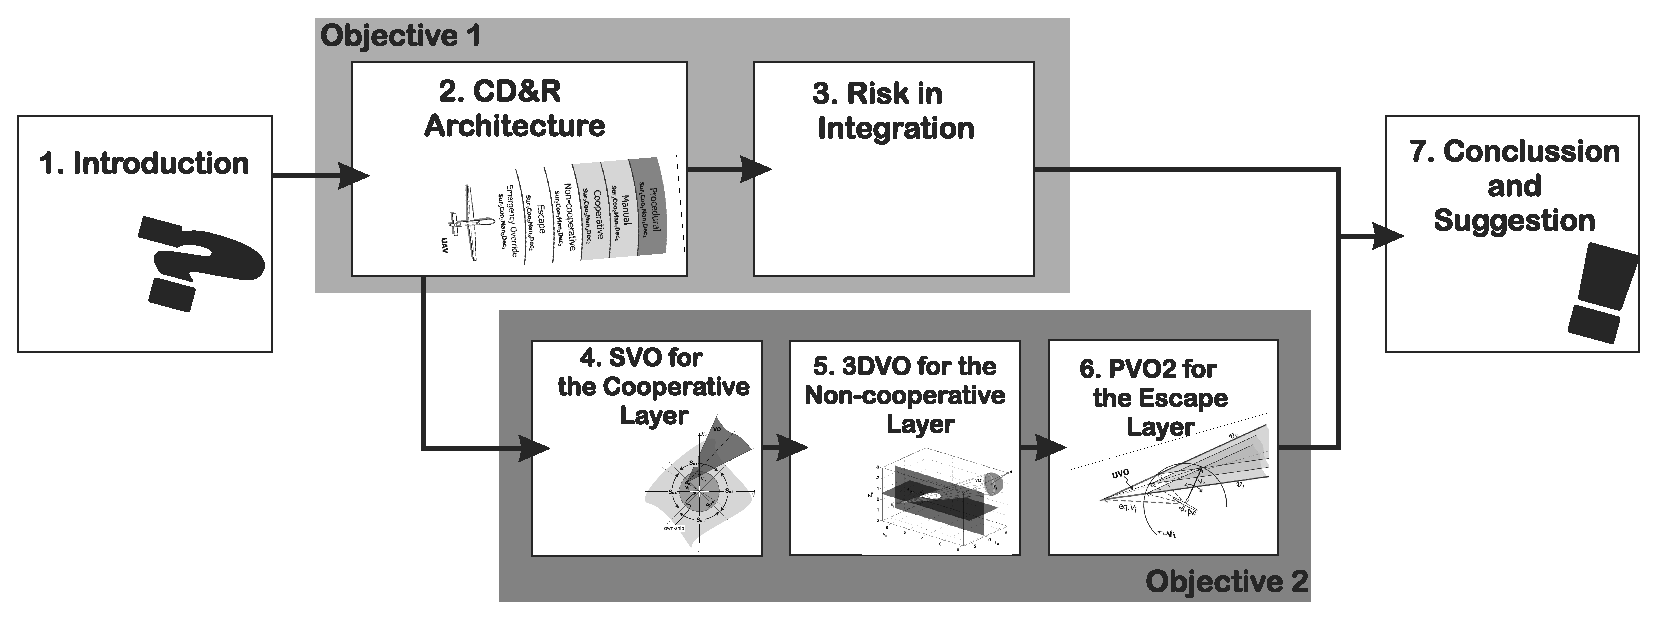
\includegraphics[width=1\textwidth]{\TheDir Figures/ThesisRoadMap}
	\caption{Structure of the chapters in the thesis and the correlation with the research objectives} 
	\label{f:ThesisRoadMap}
\end{figure}

\textbf{Chapter 1} presents the development of the novel UAV CD\&R architecture, which is based on a taxonomy of methods that define a consensus of terminology in the CD\&R system between manned and unmanned flight. Such taxonomy is produced by breaking down and recombining existing CD\&R approaches in the literature, based on their method of surveillance, coordination, maneuver, and decision. The resulting architecture consist of six layers of safety, i.e. (1) the Procedural, (2) the Manual, (3) the Cooperative, (4) Non-Cooperative, (5), the Escape, and (6) the Emergency Override, where each layer defines specific requirements that need to be fulfilled by a CD\&R system for UAVs. Each of those requirements is discussed in the end of the chapter, especially on the availability of approaches that have assessed them in the literature. 

UAV risks of collision is analyzed in \textbf{Chapter 3}, based on the implementation of the proposed architecture in an integrated airspace system. The analysis covers interaction between the different classes of UAV operation, as well as between UAVs and manned-flight. To analyze the dynamic vehicle interactions, a method called the Velocity Obstacle method (VO-method) is used, which is coupled with a set of Monte Carlo Simulations to determine the risk. 

Requirements implied by the proposed architecture that have not been sufficiently assessed in the literature are the subject of the last part of this thesis, i.e., in \textbf{Chapter 4}, \textbf{Chapter 5}, and \textbf{Chapter 6}. Three novel approaches are produced by modifying the VO-method to make it able to handle the characteristics in the selected layers of the proposed architecture, i.e., the Cooperative, Non-cooperative and Escape layer.

\textbf{Chapter 4} modifies the VO-method to incorporate a set of cooperative rules, which is adapted from manned flight Visual Flight Rules. This represents the characteristics of the Cooperative layer in the architecture. The novel method, called the Selective Obstacle method (SVO), is validated using Monte Carlo simulation for a heterogeneous conflict for up to five involved vehicles, in two-dimensional space. The chapter also set a heterogeneous simulation procedure which is use in the next chapters.

Conflicts in the Non-cooperative layer are tackled by the modification of VO-method in \textbf{Chapter 5}. Here, the VO-method is redefined to handle vehicle encounters and conflicts in a three-dimensional space, denoting the new method as 3DVO. Avoidance plane is introduced as a parameter to decide the best avoidance strategy, assuming that an agile UAV: it can maneuver in any direction in the three-dimensional space. Several heterogeneous cases are simulated in three dimensional space and incorporate a quad-rotor model as an example.

\textbf{Chapter 6} elaborate another modification of the VO-method to tackle the data uncertainties problem in the airspace. The new method, denoted as PVO2, extend further the Probabilistic Velocity Obstacle (PVO) [REF], which is already a modification from the original VO-method. The focus of the new method is to avoid as fast as possible with limited information of the counterparts. This avoidance represent the Escape layer of the architecture, where UAVs can drop its original mission in order to escape the danger.

\textbf{Chapter 7} wraps all of the chapters into an overview of results and conclusions. The chapter also provides some recommendations for further research, especially towards UAVs integration into the airspace system.

With exception the first and the last, all chapters in this thesis are based on publications in conferences and journals that were written independently and, therefore, can be read separately. Each chapter is preceded by a paragraph of introduction, that explains how the chapter is related to the overall research and the corresponding publications. The list of publications, along with the list of references, can be found after the Appendices that follows the last Chapter.



%==FIGURE


